%HW13tex
%
% Thirteenth Homework for Graduate Algebra
% Frank Sottile
%%%%%%%%%%%%%%%%%%%%%%%%%%%%%%%%%%%%%%%%%%%%%%%%%%%%%%%%%%%%%%%%%%%%%%%
\documentclass[12pt]{article}
\usepackage{multicol,amssymb,amsmath}
\usepackage{colordvi,graphicx}

%%%%%%%%%%%%%%%%%%%%%%%%%%%%%%%%  Layout     %%%%%%%%%%%%%%%%%%%%%%%%%%%%%%%%%%%%%%
\usepackage{vmargin}
\setpapersize{USletter}
\setmargrb{0.5cm}{0.05cm}{0.5cm}{0.05cm} % --- sets all four margins LTRB

\pagestyle{empty}

%%%%%%%%%%%%%%%%%%%%%%%%%%%%%%%%%%%%%%%%%%%%
\newcommand{\CC}{{\mathbb C}}
\newcommand{\FF}{{\mathbb F}}
\newcommand{\HH}{{\mathbb H}}
\newcommand{\KK}{{\mathbb K}}
\newcommand{\NN}{{\mathbb N}}
\newcommand{\QQ}{{\mathbb Q}}
\newcommand{\RR}{{\mathbb R}}
\newcommand{\TT}{{\mathbb T}}
\newcommand{\ZZ}{{\mathbb Z}}

\newcommand{\calA}{{\mathcal A}}
\newcommand{\bfe}{{\bf e}}
\newcommand{\bfi}{{\bf i}}
\newcommand{\bfj}{{\bf j}}

\newcommand{\Hom}{\mbox{Hom}}
\newcommand{\Aut}{\mbox{Aut}}
\newcommand{\End}{\mbox{End}}
\newcommand{\spec}{\mbox{spec}}
\newcommand{\cone}{\mbox{cone}}

\newcommand{\vect}[2]{(\begin{smallmatrix}#1\\#2\end{smallmatrix})}
\newcommand{\msp}{\hspace{8pt}}

\newcommand{\Square}{\raisebox{-2pt}{\includegraphics{images/Square.eps}}}


\def\Color#1#2{\special{color push cmyk #1}#2\special{color pop}}
%\def\Indigo#1{\Color{.42 1. 0. .49}{#1}}
\def\Indigo#1{\Color{1. .95 .05 .4}{#1}}
\def\MyViolet#1{\Color{.6 1. 0. .15}{#1}}


\newcommand{\barsl}{\noindent\begin{minipage}[t]{590pt}
 \Indigo{\rule{590pt}{1.2pt}}\vspace{-5.7mm}\\
\MyViolet{\rule{590pt}{1.2pt}}\vspace{-5.7mm}\\
\Blue{\rule{590pt}{1.2pt}}\vspace{-5.7mm}\\
\Green{\rule{590pt}{1.2pt}}\vspace{-5.7mm}\\
\Yellow{\rule{590pt}{1.2pt}}\vspace{-5.7mm}\\
\Orange{\rule{590pt}{1.2pt}}\vspace{-5.7mm}\\
\Red{\rule{590pt}{1.2pt}}\bigskip
\end{minipage}}


\newcommand{\barsn}{\noindent\begin{minipage}[t]{590pt}
\Indigo{\rule{590pt}{1.1pt}}\vspace{-4.5mm}\\
\MyViolet{\rule{590pt}{1.1pt}}\vspace{-4.5mm}\\
\Blue{\rule{590pt}{1.1pt}}\vspace{-4.5mm}\\
\Green{\rule{590pt}{1.1pt}}\vspace{-4.5mm}\\
\Yellow{\rule{590pt}{1.1pt}}\vspace{-4.5mm}\\
\Orange{\rule{590pt}{1.1pt}}\vspace{-4.5mm}\\
\Red{\rule{590pt}{1.1pt}}\bigskip
\end{minipage}}

\def\demph#1{\Maroon{{\sl #1}}}
\def\defcolor#1{\Maroon{#1}}

\begin{document}
\LARGE \noindent
Algebra \ \ Autumn 2023\vspace{1pt}\\
Frank Sottile\vspace{1pt}\\
\Large 27 November 2023 \hfill
\sf
 Thirteenth Homework\makebox[40pt][l]{\ }
\large\vspace{10pt}

\noindent
Write your answers neatly, in complete sentences.  
I highly recommend recopying your work before handing it in.
Correct and crisp proofs are greatly appreciated; oftentimes your work can be shortened and made clearer.

\barsl

\noindent\Maroon{{\large\sf Hand in for the grader Monday 4 December:}}
%\Blue{(Have this separate from \#?.)}\bigskip

\normalsize
\begin{enumerate}
\setcounter{enumi}{67}  %
 

%%%%%%%%%%%%%%%%%%%%%%%%%%%%%%%%%%%%%%%%%%%%%%%%%%%%%%%%%%%%%%%%%%%%%%%%%%%%%%%%%%%%%%%%%%%%%%%%%%%%
%
\item 
  Let $\FF$ be a field.
  Show that the subring $\FF[[x]][x^{-1}]$ of the 
      quotient field of $\FF[[x]]$ is a field.
      This is the field of formal Laurent series in $x$.
\vspace{-2pt}
%%%%%%%%%%%%%%%%%%%%%%%%%%%%%%%%%%%%%%%%%%%%%%%%%%%%%%%%%%%%%%%%%%%%%%%%%%%%%%%%%%%%%%%%%%%%%%%%%%%%  

%%%%%%%%%%%%%%%%%%%%%%%%%%%%%%%%%%%%%%%%%%%%%%%%%%%%%%%%%%%%%%%%%%%%%%%%%%%%%%%%%%%%%%%%%%%%%%%%%%%% 
\item The \demph{$n$th cyclotomic polynomial} is 
   \[
      f_n\ :=\ (x^n-1)/(x-1)=x^{n-1}+\dotsb+1\ \in\ \ZZ[x]\,.
   \]
          Use Eisenstein's criterion to show that if $p$ is prime, then $f_p(x+1)$ is irreducible, and deduce that $f_p$ is
          irreducible.  
%%%%%%%%%%%%%%%%%%%%%%%%%%%%%%%%%%%%%%%%%%%%%%%%%%%%%%%%%%%%%%%%%%%%%%%%%%%%%%%%%%%%%%%%%%%%%%%%%%%% 

    
%%%%%%%%%%%%%%%%%%%%%%%%%%%%%%%%%%%%%%%%%%%%%%%%%%%%%%%%%%%%%%%%%%%%%%%%%%%%%%%%%%%%%%%%%%%%%%%%%%%%  
\item     
  If $c_0,c_1,\dotsc,c_n$ are distinct elements of an integral domain $D$, and $d_0,\dotsc,d_n$ are elements of $D$, then there is at most
  one polynomial $f\in D[x]$ of degree $n$ such that $f(c_i)=d_i$ for each $i=0,\dotsc,n$.    
   
%%%%%%%%%%%%%%%%%%%%%%%%%%%%%%%%%%%%%%%%%%%%%%%%%%%%%%%%%%%%%%%%%%%%%%%%%%%%%%%%%%%%%%%%%%%%%%%%%%%%

%%%%%%%%%%%%%%%%%%%%%%%%%%%%%%%%%%%%%%%%%%%%%%%%%%%%%%%%%%%%%%%%%%%%%%%%%%%%%%%%%
 \item Show that for any ring $R$ and $R$-module $M$, $\Hom_R(R,M)\simeq (M,+,0)$, as abelian groups.
   \vspace{-2pt}
%%%%%%%%%%%%%%%%%%%%%%%%%%%%%%%%%%%%%%%%%%%%%%%%%%%%%%%%%%%%%%%%%%%%%%%%%%%%%%%%%

%%%%%%%%%%%%%%%%%%%%%%%%%%%%%%%%%%%%%%%%%%%%%%%%%%%%%%%%%%%%%%%%%%%%%%%%%%%%%%%%%
 \item  Let $R$ be a ring and $A$ be an abelian group.
   For $r\in R$ and $f\in\Hom_{\ZZ}(R,A)$, define $r.f\colon R\to A$ by $(r.f)(x)=f(xr)$ for $x\in R$.
   Show that this gives $\Hom_{\ZZ}(R,A)$ the structure of an $R$-module.
   (Part of this problem is showing that $r.f\in\Hom_{\ZZ}(R,A)$.) \vspace{-2pt}
%%%%%%%%%%%%%%%%%%%%%%%%%%%%%%%%%%%%%%%%%%%%%%%%%%%%%%%%%%%%%%%%%%%%%%%%%%%%%%%%%

%%%%%%%%%%%%%%%%%%%%%%%%%%%%%%%%%%%%%%%%%%%%%%%%%%%%%%%%%%%%%%%%%%%%%%%%%%%%%%%%%
 \item Let $R$ be a ring and $A,B,M$, and $N$ be $R$-modules.
   Let $f\in\Hom_R(A,M)$ and $g\in\Hom_R(N,B)$.
   For $\varphi\in\Hom_R(M,N)$, define $f^*(\varphi):= \varphi\circ f$ and $g_*(\varphi):=g\circ\varphi$.
   Show that these give homomorphisms of abelian groups,
   \[
   f^*\colon \Hom_R(M,N)\to\Hom_R(A,N)
   \quad\mbox{ and }\quad
   g_*\colon \Hom_R(M,N)\to\Hom_R(M,B).   \vspace{-2pt}
   \]
   Show that $f\mapsto f^*$ is a homomorphism of abelian groups $\Hom_R(A,M)\to\Hom_Z(\Hom_R(M,N),\Hom_R(A,N))$.
%%%%%%%%%%%%%%%%%%%%%%%%%%%%%%%%%%%%%%%%%%%%%%%%%%%%%%%%%%%%%%%%%%%%%%%%%%%%%%%%%

%%%%%%%%%%%%%%%%%%%%%%%%%%%%%%%%%%%%%%%%%%%%%%%%%%%%%%%%%%%%%%%%%%%%%%%%%%%%%%%%%
 \item Let $M$ be an $R$-module.
   Show that $\Hom_R(M,M)$ is a ring whose product is the composition of functions.
   It is called the \demph{endomorphism ring} of $M$, written $\mbox{End}(M)$.

   Show that $M$ is a left $\mbox{End}(M)$-module under the action by elements $f\in\mbox{End}(M)$ defined by
   $f.m=f(m)$, for $m\in M$.
   \vspace{-2pt}
%%%%%%%%%%%%%%%%%%%%%%%%%%%%%%%%%%%%%%%%%%%%%%%%%%%%%%%%%%%%%%%%%%%%%%%%%%%%%%%%%

%%%%%%%%%%%%%%%%%%%%%%%%%%%%%%%%%%%%%%%%%%%%%%%%%%%%%%%%%%%%%%%%%%%%%%%%%%%%%%%%%
 \item  An $R$-module $M$ is \demph{simple} if its only submodules are $0$ and $M$.
   Prove that every simple $R$-module is cyclic.

   Prove \demph{Schur's Lemma}, that if $M$ is simple and $M\neq 0$, then $\mbox{End}(M)$ is a division ring.
   \vspace{-2pt}
%%%%%%%%%%%%%%%%%%%%%%%%%%%%%%%%%%%%%%%%%%%%%%%%%%%%%%%%%%%%%%%%%%%%%%%%%%%%%%%%%





\end{enumerate}
%%%%%%%%%%%%%%%%%%%%%%%%%%%%%%%%%%%%%%%%%%%%%%%%%%%%%%%%%%%%%%%%%%%%%%%%%%%%%%%%%%%%%%%%%%%%%%%%%%%%

\end{document}

\noindent\Maroon{{\large\sf Hand in to Frank Monday 2 October:}}  \Blue{(Have this on a separate sheet of paper.)}
\setcounter{enumi}{15}
\begin{enumerate}
      
%%%%%%%%%%%%%%%%%%%%%%%%%%%%%%%%%%%%%%%%%%%%%%%%%%%%%%%%%%%%%%%%%%%%%%%%%%%%%%%%%%%%%%%%%%%%%%%%%%%%  
\item     
%%%%%%%%%%%%%%%%%%%%%%%%%%%%%%%%%%%%%%%%%%%%%%%%%%%%%%%%%%%%%%%%%%%%%%%%%%%%%%%%%%%%%%%%%%%%%%%%%%%%
 
\end{enumerate}  
  
\barsl
